\chapter{設計}
本章では,まずADLoggerシステムの設計概要について述べる.
ついで,クライアント側設計,サーバー側設計毎にシステム内の各モジュールについて説明する.

\section{本システムの設計概要}
本研究では,行動別時間を可視化し,必要時間を簡単に算出させるため,ADLoggerシステムを提案する.
ADLoggerは行動時間を記録し,記録された時間を元にタスク別に必要時間を予測するiOSアプリケーションである.
本システムのシステム構成図を図~\ref{fig:system}に示す.

クライアント側はタスク別時間記録モジュール,必要時間予測モジュール,表示制御モジュールから成る.

\begin{figure}[tb]
	\begin{center}
	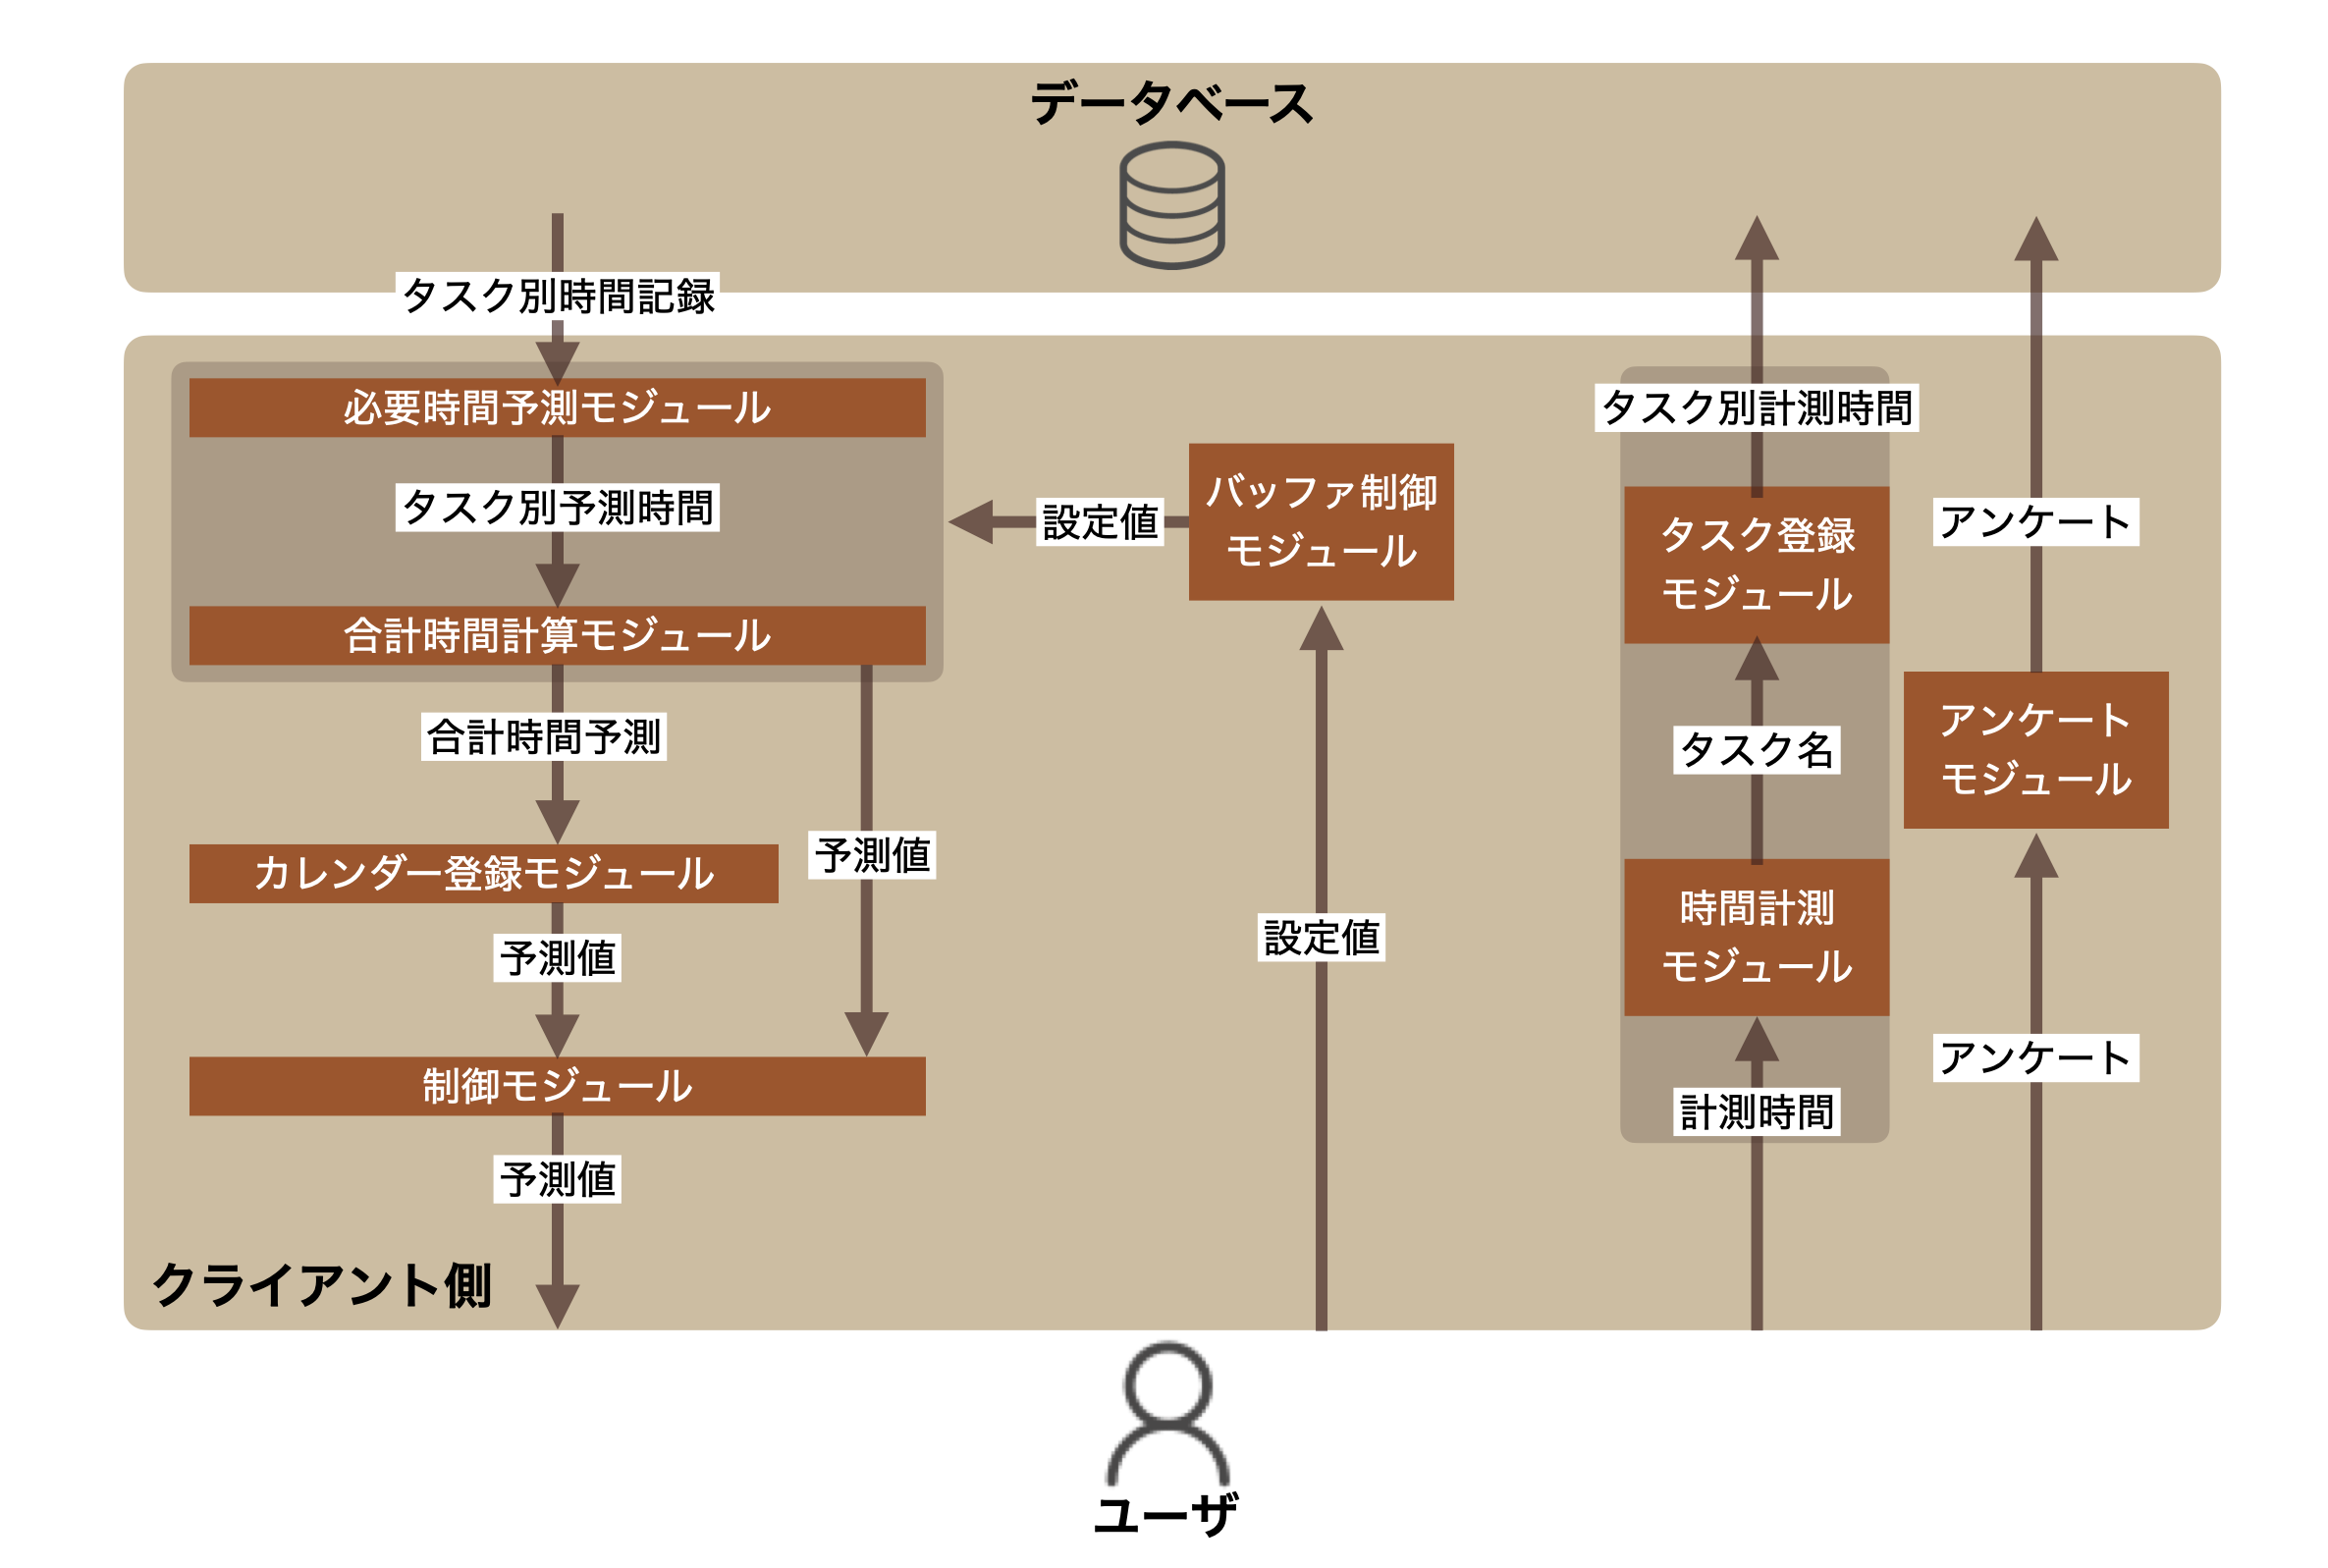
\includegraphics[width=9cm]{images/5/3.png}
	\end{center}
	\caption{システム構成図}
	\label{fig:system}
\end{figure}

\section{クライアント側設計}
本節では,クライアントであるiPhoneアプリケーションを構成する3つのモジュールについて説明する.

\subsection{タスク別時間記録モジュール}
タスク別時間記録モジュールでは,ユーザが行動した時間をタスク別に記録を行う.
ユーザは本システムを内蔵されたストップウォッチを用いて時間を測定する.
時間の測定を終了するとタスク選択画面にて行った行動を選択する.
タスク選択画面には過去入力したタスク名がリスト形式で表示されており,新規タスクである場合は新規タスク名を登録する.

\subsection{必要時間予測モジュール}
必要時間予測モジュールでは,ユーザの単一タスクないし選択された複数タスクの必要時間を予測する.
``ADLog"ボタンを押し算出画面に移動すると,タスク名毎の予測時間が自動計算されリスト形式で表示される.
リスト内のタスク名を選択すると,中央上段には選択タスクの合計必要時間が自動計算され結果が表示される.
また,同時に中央下段には合計必要時間で追加された合計バッファ時間が内訳として表示される.
それぞれの計算手法の詳細は前章にて記述した.

\subsection{表示制御モジュール}
後述する実験で精度の高い実験を行うべく,設定画面を別途設けた.
設定画面はテーブル形式であり次の2機能を操作可能とした.
\begin{enumerate}
  \item 合計時間の算出画面へのロック/ロック解除機能
  \item ストップウォッチの透明化機能
\end{enumerate}
合計時間の算出画面へのロック/ロック解除機能は``ADLog"`カラムを`OFF"にする事で``ADLog"ボタンから行動記録を見る事の制限をする事ができる.
ストップウォッチの透明化機能は``文字透明化"`カラムを` ON"にする事でストップウォッチ作動時に時間経過のカウントアップが非表示となる.
初期設定は``ADLog"`カラムを`OFF",``文字透明化"`カラムを` ON"としている.
いずれも``HELP"ボタンから閲覧できる``設定"ボタンの先にある設定画面からスイッチ形式で操作できる様にした.


\section{サーバ側設計}
サーバ側ではデータベースへの書き込み及び読み込みを行う.
ユーザ別に登録タスクとタスク時間記録をサーバ内にて管理する.

\section{まとめ}
本章では,ADLoggerシステムの設計について述べた.
次章では,本システムの実装について述べる.